\documentclass[a4paper,twocolumn]{article}

\usepackage[english]{babel}
\usepackage[utf8]{inputenc}
\usepackage{graphicx}
\usepackage{caption}

\newcommand{\D}{\mathcal{D}}
\newcommand{\T}{\mathcal{T}}
\newcommand{\X}{\mathcal{X}}
\newcommand{\Y}{\mathcal{Y}}

\title{A Survey on Transfer Learning $-$ summary}
\author{Matěj Nikl}

\begin{document}
\maketitle
As the title suggests, this paper focuses on transfer learning.
A few definitions:

\begin{itemize}
    \item a \textbf{Domain} $\D = \{\X, P(X)\}$
        \begin{itemize}
            \item a feature space $\X$
            \item a marginal probability distribution $P(X)$, where $X = \{x_1, \ldots, x_n\} \in \X$
            \item $\D_S$, $\D_T$ $-$ source and target domains
        \end{itemize}
    \item a \textbf{Task} $\T = \{\Y, f(\cdot)\}$ (given a domain $\D$)
        \begin{itemize}
            \item a label space $\Y$
            \item an objective predictive function $f(\cdot)$, which is not observed but can be learned from the training data
            \item $\T_S$, $\T_T$ $-$ source and target tasks
        \end{itemize}
    \item \textbf{Training Data} consist of pairs $\{x_i, y_i\}$
        \begin{itemize}
            \item $x_i \in \X$ and $y_i \in \Y$
            \item $D_S$, $D_T$ $-$ source and target data with $n_S$ and $n_T$ instances each
            \item In most cases $0 \le n_T \ll n_S$.
        \end{itemize}
    \item \textbf{Transfer Learning} $-$ given $\D_S$, $\T_S$, $\D_T$ and $\T_T$, transfer learning aims to help improve the learning of the target predictive function $f_T(\cdot)$ in $\D_T$ using the knowledge in $\D_S$ and $\T_S$, where $\D_S \ne \D_T$, or $\T_S \ne \T_T$
        \begin{itemize}
            \item when $\D_S = \D_T$ and $\T_S = \T_T$, the learning problem becomes a traditional machine learning problem
        \end{itemize}
\end{itemize}

In other words, transfer learning aims to extract a knowledge from one or more source tasks (and their domains) and applies the knowledge to a target task.

One should not confuse transfer learning with multi-task learning $-$ multi-task learning tries to learn all of the source and target tasks simultaneously (thus treating them all equally), transfer learning cares the most about the target task.

There are three main research issues:
\begin{enumerate}
    \item \textbf{What} to transfer $-$ which part of the knowledge can be transferred across domains or tasks $-$ some of it may be specific for individual domains or tasks, some may be common
    \item \textbf{How} to transfer $-$ learning algorithms need to be developed to transfer the knowledge
    \item \textbf{When} to transfer $-$ in which situations should transferring be done as well as in which it should not be done $-$ when source and target domains are not related to each other, transferring the knowledge may even hurt the performace $-$ a phenomenon called \textit{negative transfer}
\end{enumerate}


    % \begin{figure}[!h]
    %     \centering
    %     \frame{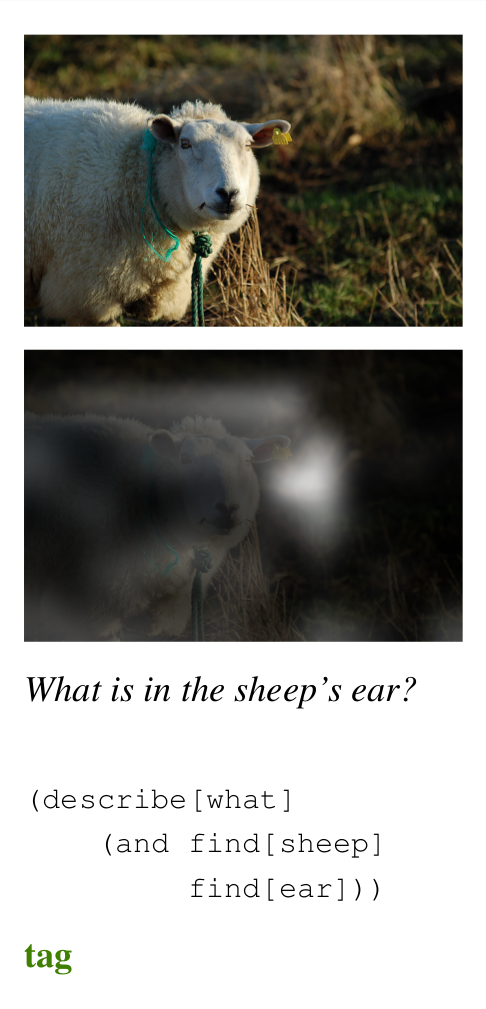
\includegraphics[width=0.4\textwidth]{sheep.png}}
    %     \frame{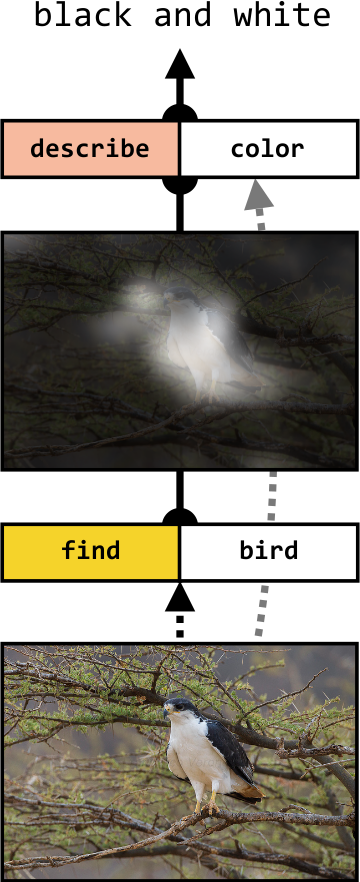
\includegraphics[width=0.4\textwidth]{bird.png}}
    %     \captionof{figure}{Examples of network instances and their computation processes}
    % \end{figure}

\subsection*{Principles of modularization}
\subsection*{Principles of growing}
NEKAM TYHLE SEKCE VECPAT OMG
\subsubsection*{Module types}

\end{document}
